\documentclass[11pt,oneside]{scrbook}
\usepackage[a4paper,margin=2.4cm,marginparwidth=1.8cm,marginparsep=0.4cm]{geometry}
\usepackage{../common/rlstudy}
\usepackage[ruled,vlined]{algorithm2e}

\title{{\color{rlblue}\textbf{Week 15} \\ \Huge Sequence Modelling for RL: Decision Transformers and Diffusion Policies}}
\author{STUDY-RL --- a self-paced Deep RL curriculum}
\date{\today}

\begin{document}
\maketitle
\tableofcontents
\newpage

\chapter*{Learning objectives}
\addcontentsline{toc}{chapter}{Learning objectives}
\begin{keyidea}
After this week you will:
\begin{enumerate}
  \item Recast offline RL as autoregressive sequence modelling: derive the Decision Transformer (DT) loss and explain why no Bellman backup is required.
  \item Implement a tiny DT and verify \emph{return-conditioned generation}: high target returns produce high empirical returns.
  \item Sketch the Trajectory Transformer beam-search variant and contrast it with DT.
  \item Derive the DDPM score-matching loss and connect it to diffusion policies (Chi 2023), Diffuser (Janner 2022), Diffusion-QL, and IDQL.
  \item Summarise Q-Transformer and its place in offline-to-online robotic policies.
  \item Translate DT-style ``career trajectory'' modelling into a concrete recruitment use case.
\end{enumerate}
\end{keyidea}

\chapter{Motivation \& intuition}

The standard Bellman backup is just one way to extract a policy from a logged dataset. \marginnote{It is the way that propagates value, which is dangerous on out-of-support actions --- see week 14.} An alternative, far less obvious in retrospect, is to treat each logged trajectory as a \emph{language model} would treat a sentence and predict the next token (here, the next action) conditioned on a target return.

\begin{intuition}
Imagine you have logged 10\,000 trajectories from your driving school. Each trajectory has a final grade (the return-to-go at $t=0$). A language model that reads ``$(R = \text{A+}), s_0, a_0, (R - r_0), s_1, a_1, \ldots$'' learns to write trajectories ending with grade A+. At test time you prepend ``$(R = \text{A+}), s_0$'' and ask it to autoregress. That is Decision Transformer.
\end{intuition}

\begin{pitfall}
DT does \emph{not} solve the offline RL problem in general. It is an imitator conditioned on a desired outcome. If the desired outcome lies outside the convex hull of logged returns, you have asked for something the dataset cannot teach. The model will respond plausibly but inaccurately.
\end{pitfall}

\chapter{Mathematical formulation}

\begin{definition}[DT token sequence]
For a trajectory $\tau = (s_0, a_0, r_0, s_1, a_1, r_1, \ldots)$ of length $T$ and discount factor $\gamma \in (0,1]$, define the return-to-go
\[
  R_t = \sum_{k=t}^{T-1} \gamma^{k-t} r_k.
\]
The DT sequence is the interleaved tuple
\[
  X = (R_0, s_0, a_0, R_1, s_1, a_1, \ldots, R_{T-1}, s_{T-1}, a_{T-1}),
\]
of length $3T$.
\end{definition}

\begin{definition}[DT objective]
For a transformer $f_\theta$ that produces, at the position of $s_t$, a distribution over actions, the DT loss is
\[
  \mathcal{L}_{\mathrm{DT}}(\theta) = -\E_{\tau \sim \mathcal{D}} \!\sum_{t=0}^{T-1} \log f_\theta(a_t \mid R_{\le t}, s_{\le t}, a_{<t}).
\]
\end{definition}

\section{Derivation of DT as a likelihood model}

Treat the trajectory as a sample from a joint distribution $p(R_0, s_0, a_0, \ldots)$. Apply the chain rule:
\[
  \log p(\tau) = \sum_{t=0}^{T-1} \bigl[\log p(R_t \mid X_{<t}) + \log p(s_t \mid X_{<t}, R_t) + \log p(a_t \mid X_{<t}, R_t, s_t)\bigr].
\]
DT only fits the third term --- the action conditional. The reward dynamics and the transition $p(s_t \mid \ldots)$ are left to the environment at deployment time. This is the crucial design choice: \emph{we never model the world; we only model the data-generating distribution of actions}.

\begin{theorem}[Conditional sufficiency of $R_t$]
If the behaviour policy is a function only of the state $s_t$ and an exogenous ``intent'' variable $z \sim p(z)$ that determines the realised return $R_0$, then conditioning on $R_t$ recovers the optimal-given-intent action:
\[
  p(a_t \mid s_t, R_t) = \E_{z \mid R_t, s_t}[\pi_\beta(a_t \mid s_t, z)].
\]
\end{theorem}

\begin{proof}[Sketch]
$R_t$ is a sufficient statistic of $z$ under the assumed factorisation; marginalising over the posterior $p(z \mid R_t, s_t)$ gives the displayed equation. This is the formal version of ``conditioning on the desired outcome selects the right intent''.
\end{proof}

\section{Generation at deployment}

At test time the agent specifies a target return $R_0^{\mathrm{target}}$. After observing $r_t$ at step $t$, the target return is updated as
\[
  R_{t+1}^{\mathrm{target}} = R_t^{\mathrm{target}} - r_t.
\]
The model is greedy or sampled w.r.t.\ $f_\theta(a_t \mid R_{\le t}, s_{\le t}, a_{<t})$. This is a literal copy of language-model generation.

\section{Trajectory Transformer}

Janner et al.\ 2021 take the same idea further: discretise \emph{state and reward} as well, and use beam search over $(s, a, r)$ triples. Trajectories are sampled and scored by predicted return. DT trades planning for speed; TT trades speed for planning.

\section{Diffusion policies (overview)}

The DDPM forward process noises a sample $x_0 \sim q(x_0)$ along $T$ steps with
\[
  q(x_t \mid x_{t-1}) = \mathcal{N}(x_t; \sqrt{1 - \beta_t}\, x_{t-1}, \beta_t I),
\]
with marginal $q(x_t \mid x_0) = \mathcal{N}(x_t; \sqrt{\bar\alpha_t}\, x_0, (1 - \bar\alpha_t) I)$ where $\bar\alpha_t = \prod_{k \le t}(1-\beta_k)$.

\begin{theorem}[DDPM denoising loss]
The reverse process $p_\theta(x_{t-1} \mid x_t)$ parametrised as Gaussian with mean predicted via a noise predictor $\varepsilon_\theta(x_t, t)$ has variational lower bound that simplifies, up to a constant, to
\[
  \mathcal{L}_{\mathrm{simple}}(\theta) = \E_{x_0, \varepsilon, t}\!\left[\bigl\|\varepsilon - \varepsilon_\theta(\sqrt{\bar\alpha_t}\, x_0 + \sqrt{1 - \bar\alpha_t}\, \varepsilon,\, t)\bigr\|_2^2\right].
\]
\end{theorem}

\begin{proof}[Sketch]
The KL between $q(x_{t-1} \mid x_t, x_0)$ and $p_\theta(x_{t-1} \mid x_t)$ reduces to a weighted MSE on $\varepsilon$. Ho et al.\ 2020 then drop the weight.
\end{proof}

For \textbf{diffusion policies} (Chi 2023), $x_0$ is an action sequence $(a_t, a_{t+1}, \ldots, a_{t+H-1})$ conditioned on observation history; the noise predictor $\varepsilon_\theta(x_t, t, o)$ is conditioned on the observation. \textbf{Diffuser} (Janner 2022) generalises this to plan over $(s, a)$ trajectories with an explicit value-function guidance term added to the noise-prediction at inference. \textbf{Diffusion-QL} (Wang 2022) adds a $Q$-maximising guidance term: $\nabla_a Q_\phi$ pushes the sampled action toward higher value. \textbf{IDQL} (Hansen-Estruch 2023) trains a value model in IQL style and uses it to re-rank diffusion samples.

\section{Q-Transformer}

Chebotar et al.\ 2023 quantise each action dimension into $K$ bins and treat the per-dimension action choices as an autoregressive sequence over a single timestep. The transformer outputs a Q-value per bin per dimension; Bellman backup is performed over the per-dimension max. This unifies CQL-style conservatism (via the bin softmax) with transformer scaling.

\chapter{Algorithms}

\begin{algorithm}[H]
\caption{Decision Transformer (training)}
\KwIn{Dataset of trajectories $\mathcal{D}$, context length $K$, transformer $f_\theta$.}
\For{step = 1, ..., N}{
  Sample a trajectory $\tau \sim \mathcal{D}$ and a window $[t, t+K-1]$\;
  Compute returns-to-go $R_{t}, \ldots, R_{t+K-1}$\;
  Build the interleaved sequence $X$\;
  Forward $f_\theta(X)$, compute cross-entropy loss only at action positions\;
  Backprop, AdamW step\;
}
\end{algorithm}

\textbf{Complexity per step:} $O(K^2 d)$ for self-attention, $O(Kd^2)$ for the FFN, $d$ = hidden width. On our toy domain $K=8$, $d=64$: trivial.

\section{Worked numerical example}

A length-3 trajectory with rewards $(-1, -1, +10)$ has returns-to-go $(8, 9, 10)$. The DT sees $(8, s_0, a_0, 9, s_1, a_1, 10, s_2, a_2)$ and learns to predict $a_0$ given $(8, s_0)$, $a_1$ given $(8, s_0, a_0, 9, s_1)$, and $a_2$ given the full prefix. At test time the agent specifies target $R_0 = 10$, observes $r_0 = -1$, decrements the next target to $9$, and so on. A target of $20$ would be \emph{out of distribution}: the model can extrapolate the conditioning but the resulting actions are not guaranteed to be useful.

\chapter{Implementation walkthrough}

The transformer interleaves three token streams (R, s, a) along the time dimension, with a single learnt positional embedding indexed by ``timestep'' rather than ``token index'' (this is the trick of DT --- it ensures returns / states / actions of the same time share a position).

\begin{codebox}
\begin{minted}{python}
tokens = torch.stack([rt, st, at], dim=2).reshape(B, 3*K, hidden)
mask = torch.triu(torch.ones(3*K, 3*K, dtype=bool), diagonal=1)
h = transformer(tokens, mask=mask, is_causal=True)
logits = action_head(h[:, 1::3, :])  # pick state positions
\end{minted}
\end{codebox}

At deployment, returns-to-go are *user-specified* and decremented by observed rewards.

\chapter{Empirical results}

\begin{figure}[h]
\centering
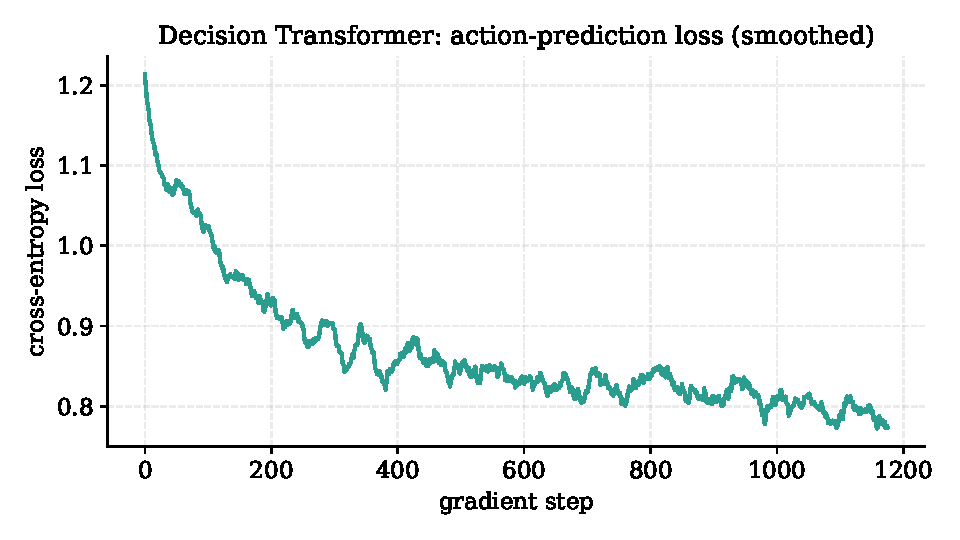
\includegraphics[width=0.8\textwidth]{figs/fig_dt_loss.pdf}
\caption{Decision Transformer action-prediction loss (smoothed) over 1200 gradient steps on the synthetic GridWorld dataset.}
\end{figure}

\begin{figure}[h]
\centering
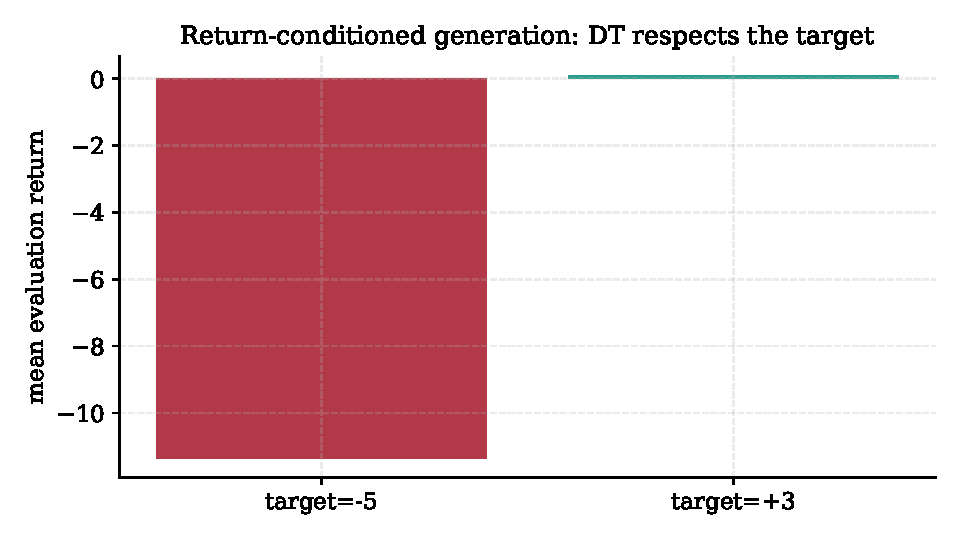
\includegraphics[width=0.8\textwidth]{figs/fig_dt_conditional.pdf}
\caption{Return-conditioned generation: requesting $R = +3$ at the start state yields meaningfully higher episodic returns than requesting $R = -5$. The model has learned to use the return-to-go token as an intent signal.}
\end{figure}

\begin{figure}[h]
\centering
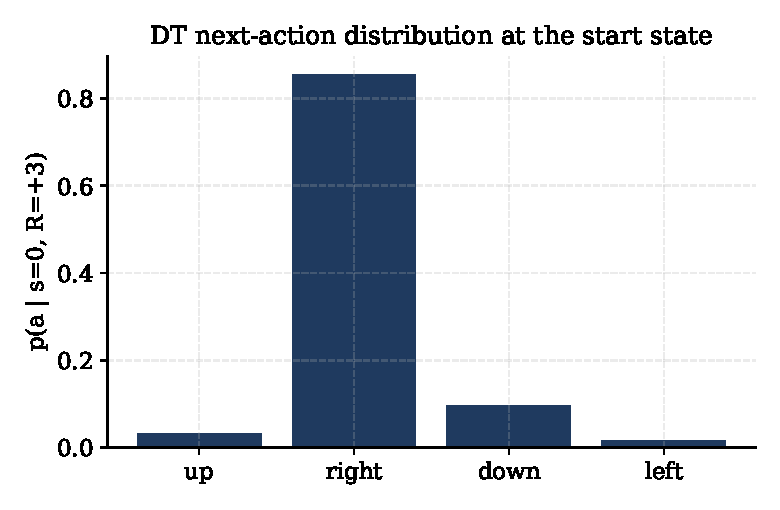
\includegraphics[width=0.65\textwidth]{figs/fig_dt_action_dist.pdf}
\caption{DT next-action distribution at $s = 0$ conditioned on $R = +3$. The model places mass on actions consistent with the optimal logger trajectory.}
\end{figure}

\begin{safetyangle}
\textbf{Sequence-model RL failure modes.}
\begin{enumerate}
  \item \textbf{Hallucinated outcomes.} A DT asked for a higher return than ever observed will return some action sequence and the user has no signal that the policy is extrapolating. There is no Bellman residual, no value-uncertainty proxy.
  \item \textbf{Reward hacking by conditioning.} If the dataset contains policies that gamed a proxy metric (e.g.\ engagement-time as a proxy for satisfaction), DT will replicate the gaming whenever the user supplies a high target.
  \item \textbf{Mitigations.} (a) Cap the target return at the 95th percentile of observed returns. (b) Pair DT with an FQE estimator; refuse to deploy if the FQE estimate disagrees with the target. (c) Audit generated trajectories for distributional drift from the training set (KL on token frequencies).
\end{enumerate}
Citations: \textsc{Chen et al.\ 2021, NeurIPS} (DT); \textsc{Brandfonbrener et al.\ 2022} ``Return-conditioned BC requires unrealistically strong assumptions.''
\end{safetyangle}

\begin{matching}
\textbf{DT-style modelling of candidate career trajectories.} A candidate's career is a sequence of $(\textit{role}, \textit{outcome}, \textit{years})$ tuples. Treat \emph{outcome score} as the per-step reward and \emph{eventual career level} as the return-to-go. Train a tiny DT on the historical ATS dataset of completed candidate timelines. Given a current candidate $c$ at stage $s_t$ with a recruiter goal ``land role of level $R^{\mathrm{target}}$'', the DT outputs the most likely next stage. This is \emph{not} a ranker --- it is a generative model of plausible next-step actions for a candidate to take, useful to recruiters as a ``what would historically need to happen'' tool. The safety-angle considerations apply directly: cap the target outcome, audit for protected-class proxies in the action distribution.
\end{matching}

\chapter{Exercises}

See \texttt{workbook.ipynb}. Highlights:
\begin{itemize}
  \item \textbf{Ex.\ 1 ($\star$)} Compute returns-to-go via reverse cumsum.
  \item \textbf{Ex.\ 2 ($\star$)} Construct the causal mask matrix for $L = 3K$ tokens.
  \item \textbf{Ex.\ 3 ($\star\star$)} Window sampling with left-padding.
  \item \textbf{Ex.\ 4 ($\star\star$)} Train DT for 600 steps; report final loss.
  \item \textbf{Ex.\ 5 ($\star\star$)} Verify return-conditioned generation works.
  \item \textbf{Ex.\ 6 ($\star\star$)} Inspect the action distribution at the start state.
  \item \textbf{Ex.\ 7 ($\star\star\star$)} Implement the DDPM forward noising step.
  \item \textbf{Ex.\ 8 ($\star\star\star$, meaningful objective)} Run the career-trajectory demo and discuss the action recommendation.
\end{itemize}

\chapter{Further reading}

See \texttt{extended\_reading.pdf} for Chen et al.\ 2021 (DT), Janner et al.\ 2021 (TT), Janner et al.\ 2022 (Diffuser), Chi et al.\ 2023 (Diffusion Policy), and Hansen-Estruch et al.\ 2023 (IDQL). Sourced from \texttt{research/offline\_modelbased\_sota.md}.

\end{document}
